\documentclass[12pt]{article}
\usepackage[utf8]{inputenc}
\usepackage[T1]{fontenc}
\usepackage[a4paper, left=2.4cm, right=2.4cm, top=2cm, bottom=2cm, nomarginpar]{geometry}
\usepackage{amsmath, algorithm, pgfplots, pgf, pdfpages, amsfonts, amssymb, stmaryrd, enumitem,graphicx, algpseudocode, setspace, listings, courier, color, caption, centernot, hyperref, lstautogobble, zi4, mathtools, lmodern, colortbl, array, multicol, fancyhdr, lastpage, svg}
\usepackage{booktabs}
\hypersetup{
    pdftitle={CE204_FP1_G6},
    pdftoolbar=true,        % show Acrobat’s toolbar?
    pdfmenubar=true,        % show Acrobat’s menu?
    pdfauthor={Muhammet Yağcıoğlu},
    pdfsubject={CE204_FP_RPs},
    pdfcreator={Muhammet Yağcıoğlu},   % creator of the document
    pdfproducer={Muhammet Yağcıoğlu}, % producer of the document
    colorlinks,
    linkcolor={black},
    citecolor={black},
    urlcolor={blue!80!black}
}
\usepackage[noblocks]{authblk}
\usepackage[version=4]{mhchem}
\usepackage[export]{adjustbox}
\usepackage{eso-pic} % Required for absolute positioning
\graphicspath{ {./images/} }
\usetikzlibrary{patterns}
\usepackage{tikz-3dplot}
\usepackage[version=4]{mhchem}
\usepackage[export]{adjustbox}
\usepgfplotslibrary{groupplots}
\usepackage{xcolor}
\usepackage[absolute,overlay]{textpos}
\usepackage{ragged2e}
\usepackage{xcolor}
\usepackage{amsthm}
\usepackage{tikz}




%----------compiler settings---------
\setlength{\parindent}{0pt}
\everymath{\displaystyle}
\onehalfspacing

%-----------colors----------
\pgfplotsset{compat=1.18}
\definecolor{bluekeywords}{rgb}{0.13, 0.13, 1}
\definecolor{greencomments}{rgb}{0, 0.5, 0}
\definecolor{redstrings}{rgb}{0.9, 0, 0}
\definecolor{graynumbers}{rgb}{0.5, 0.5, 0.5}
\definecolor{bronze}{rgb}{0.82, 0.41, 0.12}
\definecolor{crimson}{rgb}{0.86, 0.08, 0.24}
\definecolor{brown(web)}{rgb}{0.65, 0.16, 0.16}
\definecolor{darkspringgreen}{rgb}{0.16, 0.32, 0.75}
\definecolor{blue(ncs)}{rgb}{0.0, 0.53, 0.74}
\definecolor{amber}{rgb}{1.0, 0.49, 0.0}
\definecolor{cadmiumgreen}{rgb}{0.0, 0.42, 0.24}




%-------code frame-----------
\lstset{
    autogobble,
    columns=fullflexible,
    showspaces=false,
    showtabs=false,
    breaklines=true,
    showstringspaces=false,
    breakatwhitespace=true,
    escapeinside={(*@}{@*)},
    commentstyle=\color{greencomments},
    keywordstyle=\color{bluekeywords},
    stringstyle=\color{redstrings},
    numberstyle=\color{graynumbers},
    basicstyle=\ttfamily\footnotesize,
    frame=l,
    framesep=12pt,
    xleftmargin=12pt,
    tabsize=4,
    captionpos=b
}



\lstdefinelanguage{myMMA}{
keywords={SetDirectory, NotebookDirectory, Exp, IdentityMatrix, Eigenvalues, 
ListPlot, PlotRange, PlotStyle, Directive, PointSize, AspectRatio, Blue, Graphics, Line, 
Manipulate, Show, Sqrt, UniformDistribution, GammaDistribution, BetaDistribution, 
Nintegrate, For, DataRange, AxesLabel, PlotLabel, Transpose, Export, Plot, Append, Infinity},
keywordstyle=\color{black},
commentstyle=\color{gray}, 
identifierstyle=\color{blue},
sensitive=false,
comment=[l]{(*},
morecomment=[s]{/*}{*/},
morestring=[b]',
morestring=[b]"
}






%-----gauss declare---------
\pgfmathdeclarefunction{gauss}{2}{%
  \pgfmathparse{1/(#2*sqrt(2*pi)) * exp(-((x-#1)^2)/(2*#2^2))}%
}
\usetikzlibrary{arrows.meta, decorations.markings}
\pgfplotsset{compat=1.17}







%--------------page numbering------------
\fancyfoot[R]{page \thepage\ of \textcolor{bronze}{\pageref{LastPage}}}
\fancyhead[R]{Group 6}



%-------------qframe settings---------------

\usepackage[framemethod=TikZ]{mdframed}
\newmdenv[%
    skipabove=1em, % space above the frame
    skipbelow=1em, % space below the frame
    linewidth=1pt, % width of the frame lines
    linecolor=gray!80, % color of the frame lines
    backgroundcolor=gray!9, % background color inside the frame
    roundcorner=5pt, % radius of the rounded corners
    innerleftmargin=1em, % margin within the frame at the left
    innerrightmargin=1em, % margin within the frame at the right
    innertopmargin=0.5em, % margin within the frame at the top
    innerbottommargin=0.5em % margin within the frame at the bottom
]{qframe}

\newenvironment{q}
{
    \begin{qframe}
    \noindent\textit{\textbf{Problem Statement:}}
    \par\smallskip
}
{
    \end{qframe}
}





%-------------ANSWER TAG---------------
\newcommand{\AnswerTag}{\hfill 
\begin{tikzpicture} \fill[black] (0.35cm,0) -- (0,0.175cm) -- (0.35cm,0.35cm) -- cycle;\end{tikzpicture}}



%-------Theorem and another question frames----------
\newenvironment{theorem}{\begin{mdframed}\textbf{Theorem.}}{\end{mdframed}}

%usage: \begin{theorem}

\newenvironment{question}{\begin{mdframed}\textbf{Question.}}{\end{mdframed}}

%usage: %usage: \begin{question}
\fancyhead[L]{CE 224 Mechanics of Materials, Fall 2023, Homework-4 }
\title{\vspace{-1cm}CE 224 - HW4}
\author{Muhammet Yağcıoğlu - 290204042}
\usepackage{hyperref} 
\begin{document}
\maketitle\thispagestyle{fancy}
\pagestyle{fancy}
\tableofcontents
\newpage



\section*{Question 1}
\addcontentsline{toc}{section}{Question 1}
\begin{q}
1. For the beam showing in the figure, consider section \(\boldsymbol{n}-\boldsymbol{n}\) and determine;
(a) The largest shearing stress in that section

(b) The shearing stress at point \(a\).
\end{q}
\begin{figure}[!ht]
    \centering
    \resizebox{0.7\textwidth}{!}{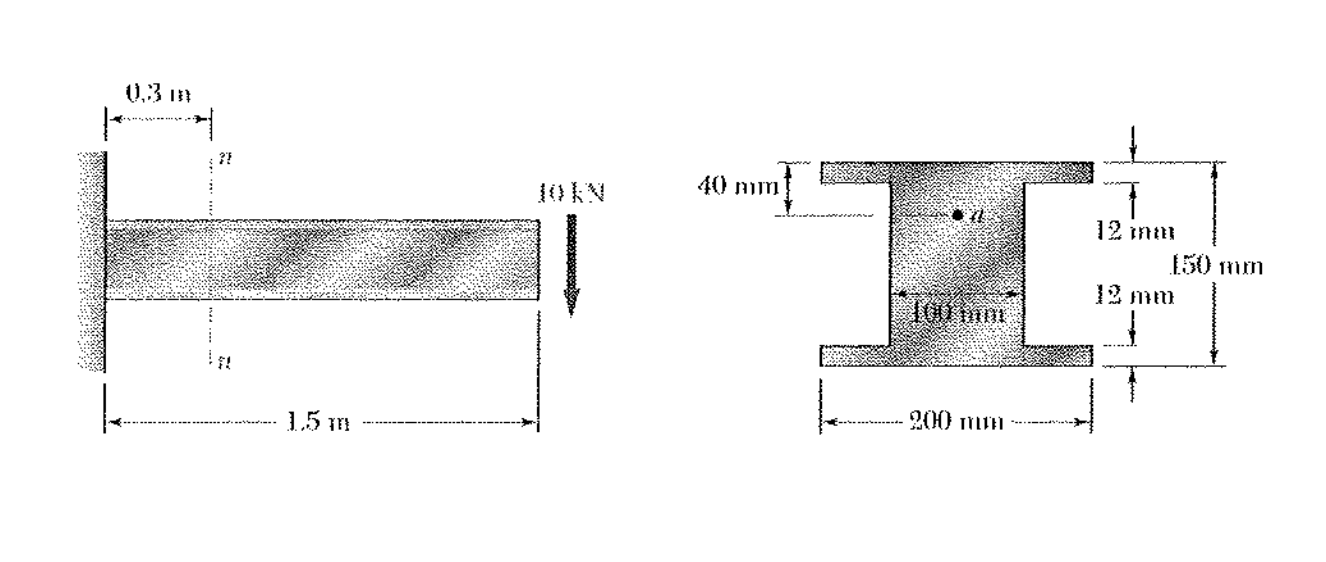
\includegraphics{image.png}}
    \caption{}
    \label{fig:enter-label}
\end{figure}

Define the composite beam as consisting of multiple sections with individual geometries. Denote the dimensions of each section by \( b_i \) and \( h_i \), with \( i \) indexing the section. The moment of inertia for a rectangular section is given by \( \frac{1}{12} b_i h_i^3 \). For a composite beam, the total moment of inertia \( I \) is the sum of the individual moments, taking into account the parallel axis theorem if necessary. Thus, for a beam composed of different sections, we have:
\[ I = \sum_{i} \left( \frac{1}{12} b_i h_i^3 + A_i d_i^2 \right), \]

where \( A_i \) is the area of the section, and \( d_i \) is the distance from the centroid of the section to the centroid of the entire cross-section. If we calculate

\[
\begin{aligned}
I & =I_1+4 I_2 \\
& =\frac{1}{12} b_1 h_1^3+4\left(\frac{1}{12} b_2 h_2^3+A_2 d_2^2\right), \\
& =\frac{1}{12}(100)(150)^3+4\left[\left(\frac{1}{12}\right)(50)(12)^3+(50)(12)(69)^2\right], \\
& =28.125 \times 10^6+4\left[0.0072 \times 10^6+2.8566 \times 10^6\right], \\
& =39.58 \times 10^6 \mathrm{~mm}^4=39.58 \times 10^{-6} \mathrm{~m}^4.
\end{aligned}
\]

The first moment of area \( Q \) for any point in the cross-section is calculated by summing the products of the area of each section above (or below) the point of interest and the distance from the centroid of that section to the point of interest. So, for a point at a distance \( y \) from the neutral axis, \( Q \) is given by:
\[ Q = \sum_{i} A_i \bar{y}_i, \]

where \( \bar{y}_i \) is the distance from the centroid of section \( i \) to the point of interest.

\begin{figure}[!ht]
    \centering
    \resizebox{0.7\textwidth}{!}{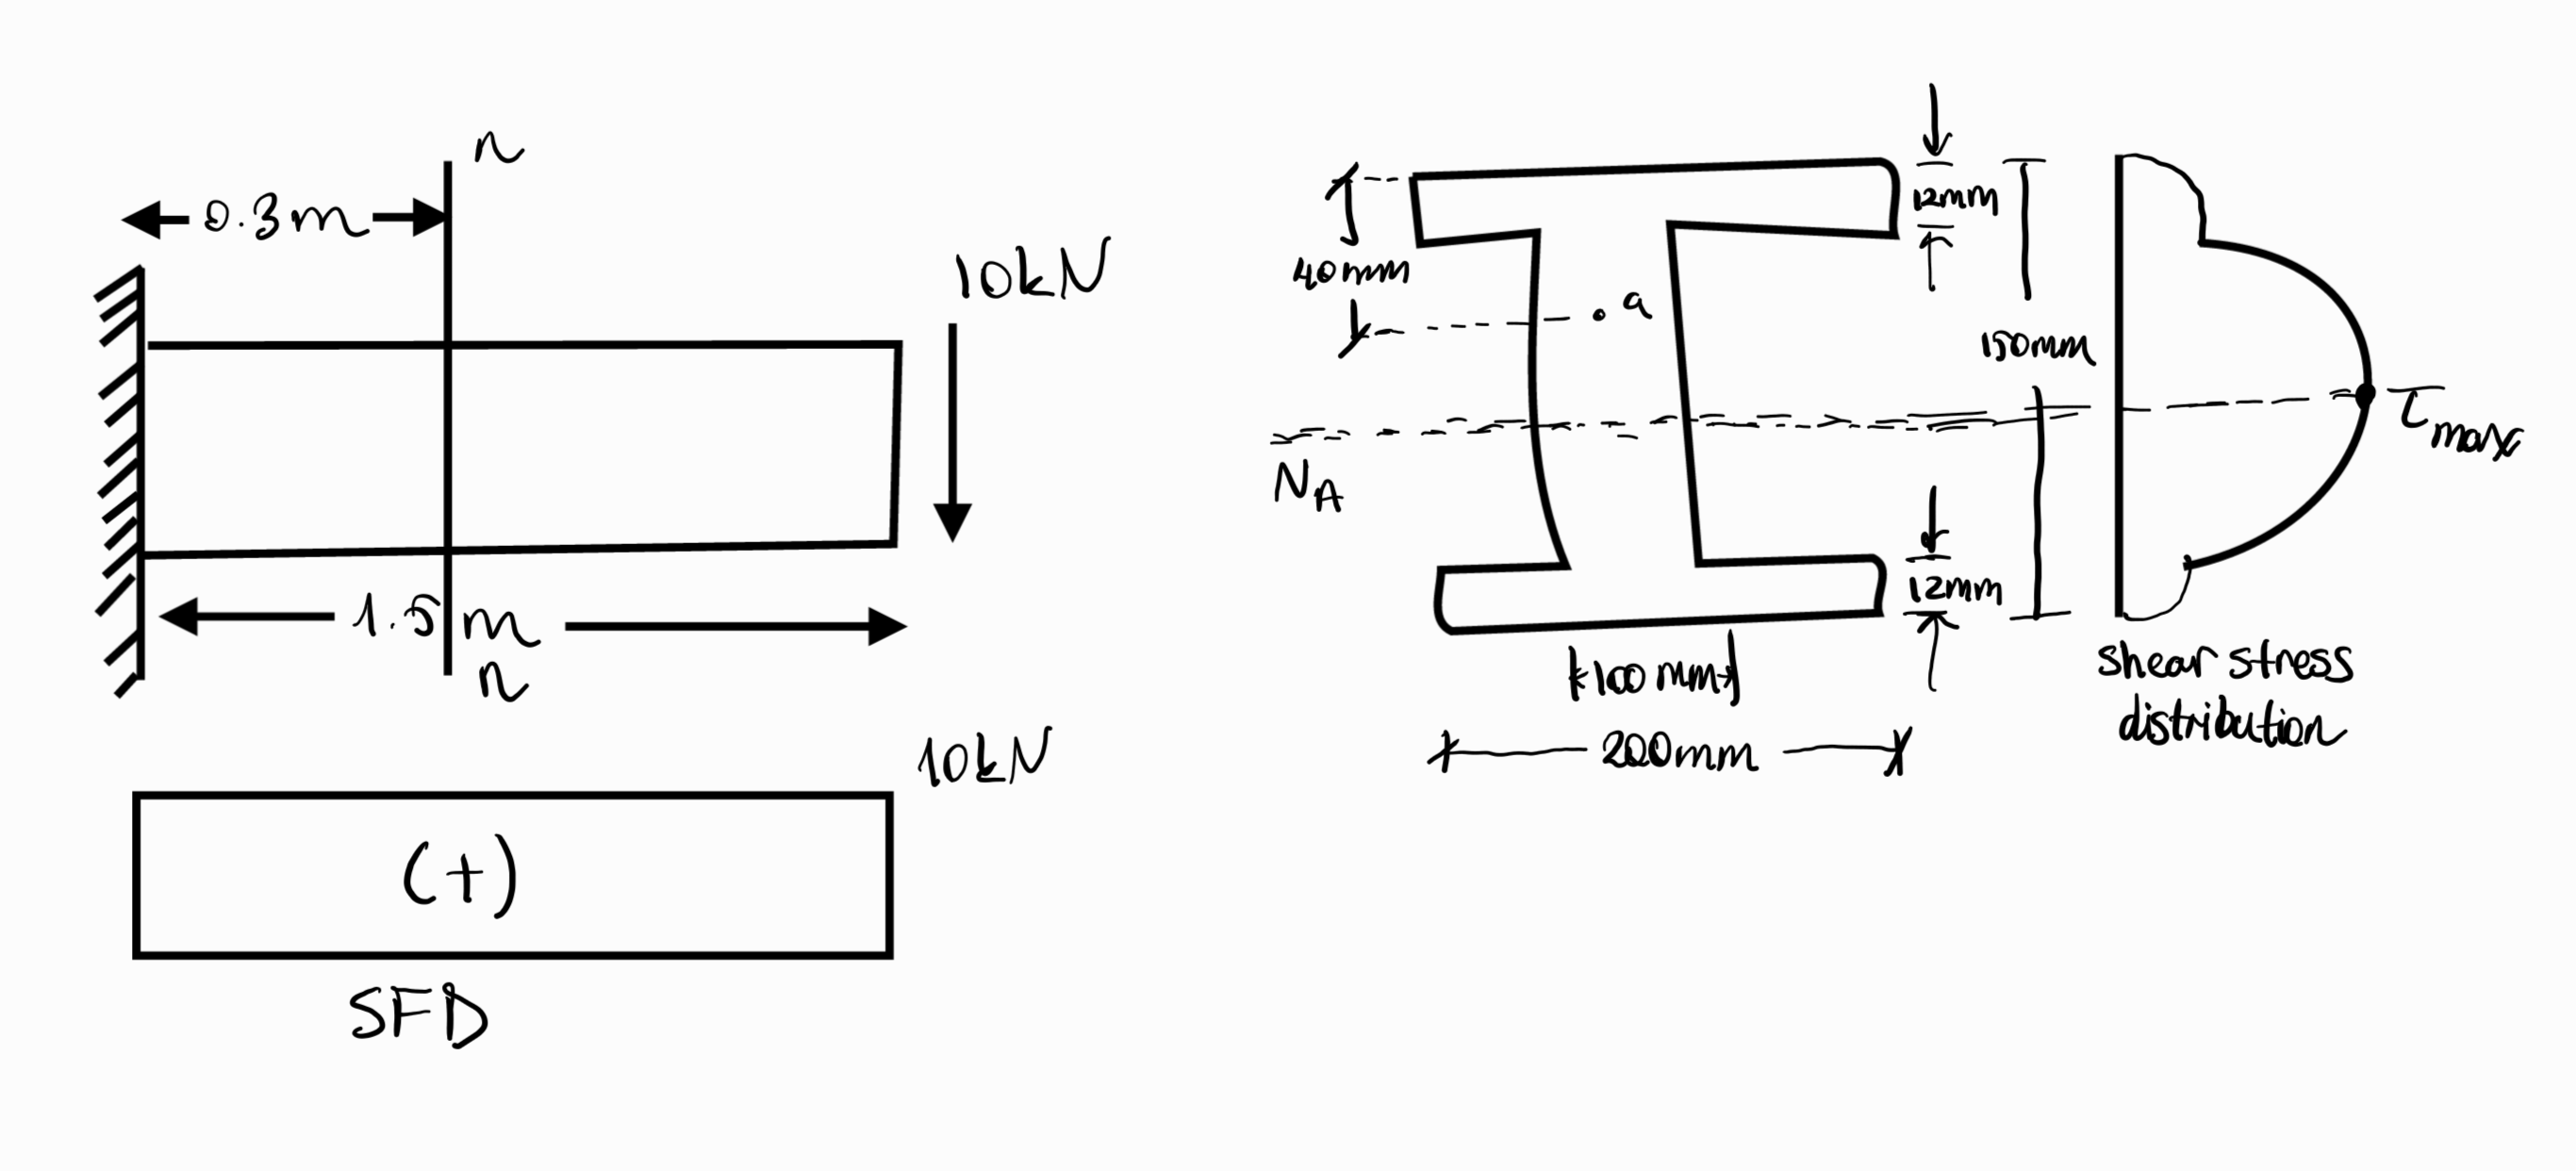
\includegraphics{Screenshot_20231214_212731_Samsung Notes.png}}
    \caption{}
    \label{fig:enter-label}
\end{figure}


Thus, for each part:

\subsection*{Part a}
\addcontentsline{toc}{section}{Part a}

\[
\begin{aligned}
Q & =A_1 \bar{y}_1+2 A_2 \bar{y}_2, \\
& =(100)(75)(37.5)+(2)(50)(12)(69), \\
& =364.05 \times 10^3 \mathrm{~mm}^3=364.05 \times 10^{-6} \mathrm{~m}^3, \\
t & =100 \mathrm{~mm}=0.100 \mathrm{~m}, \\
\tau_{\max } & =\frac{V Q}{I t}=\frac{\left(10 \times 10^3\right)\left(364.05 \times 10^{-6}\right)}{\left(39.58 \times 10^{-6}\right)(0.100)}=920 \times 10^3 \mathrm{~Pa}.
\end{aligned}
\]
\AnswerTag

\subsection*{Part b}
\addcontentsline{toc}{section}{Part b}

\[
\begin{aligned}
Q & =A_1 \bar{y}_1+2 A_2 \bar{y}_2, \\
& =(100)(40)(55)+(2)(50)(12)(69), \\
& =302.8 \times 10^3 \mathrm{~mm}^3=302.8 \times 10^{-6} \mathrm{~m}^3, \\
t & =100 \mathrm{~mm}=0.100 \mathrm{~m}, \\
\tau_a & =\frac{V Q}{I t}=\frac{\left(10 \times 10^3\right)\left(302.8 \times 10^{-6}\right)}{\left(39.58 \times 10^{-6}\right)(0.100)}=765 \times 10^3 \mathrm{~Pa}.
\end{aligned}
\]

\AnswerTag

\vfill
\begin{flushright}
\textbf{ans.} \(\tau_{\max }=920 \times 10^3 \mathrm{~Pa}, \tau_a= 765 \times 10^3 \mathrm{~Pa}.\)
\end{flushright}

\newpage
\section*{Question 2}
\addcontentsline{toc}{section}{Question 2}
\begin{q}
The beam shown in cross section is fabricated by joining two \(150-\mathrm{mm}\) by \(150-\mathrm{mm}\) wooden boards with 20-mm-thick plywood strips. Knowing that the working shear stress for plywood is \(2 \mathrm{MPa}\), determine the maximum allowable vertical shear force that can be carried by the beam.
\end{q}
\begin{figure}[!ht]
    \centering
    \resizebox{0.6\textwidth}{!}{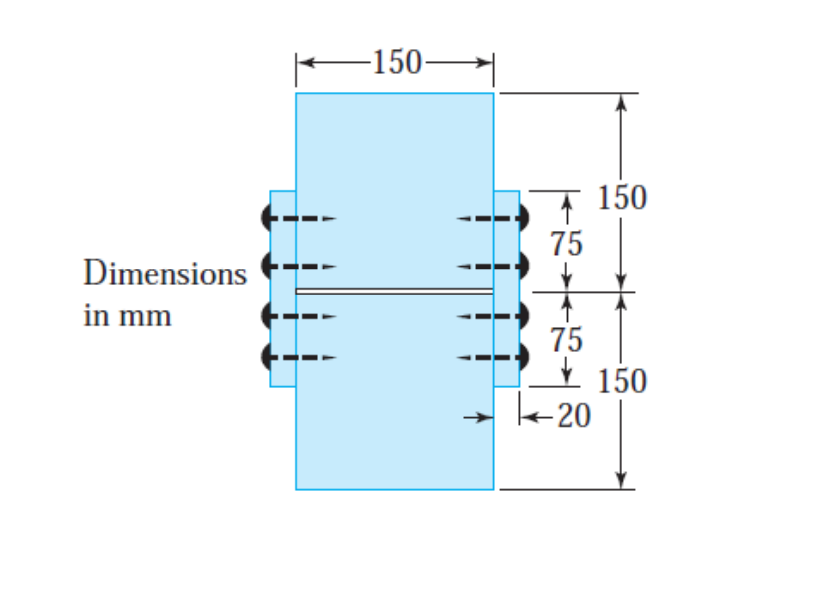
\includegraphics{Screenshot 2023-12-14 214653.png}}
    \caption{}
    \label{fig:enter-label}
\end{figure}



Let the cross-sectional dimensions of the wooden boards be \(a = 150 \, \text{mm}\) and \(b = 150 \, \text{mm}\), and the thickness of the plywood strip be \(t = 20 \, \text{mm}\). The composite cross-section can be viewed as a single rectangular section with effective width \(b_{\text{eff}} = a + 2t\). The moment of inertia, \(I\), for this rectangular cross-section about its neutral axis (which passes through the centroid and is perpendicular to the width) is computed using the standard formula for a rectangle: \(I = \frac{1}{12} b_{\text{eff}} h^3\), where \(h\) is the height of the rectangle, which, in this case, is \(b\). Substituting the given values, we find:

\[
I = \frac{1}{12} (150 \times 300^3  \, \text{mm}^3) + \frac{1}{12}(150^3 \times 40 \, \text{mm})= 1.80 \times 10^{-3} \, \mathrm{~m}^3.
\]

\[
 V=\frac{\tau_w l b}{Q}
\]

Given that the working shear stress for plywood is \(\tau = 2 \, \text{MPa}\), we set this as the maximum shear stress.


\[
\begin{aligned}
& \mathrm{\tau}_{\mathrm{w}}=2 \times 10^6 \mathrm{~Pa} \\
& \mathrm{l}=348.75 \times 10^{-6} \mathrm{~m}^2 \\
& \mathrm{Q}=1.8 \times 10^{-3} \mathrm{~m}^3 \\
& \mathrm{~B}=0.04 \mathrm{~m} \\
& \mathrm{~V}=\left(2 \times 10 \frac{\mathrm{N}}{\mathrm{m}^2}\right)\left(348.75 \times 10^{-6} \mathrm{~m}^2\right)(0.04 \mathrm{~m})\left(1.8 \times 10^{-3} \mathrm{~m}^3\right) \\
& \quad=15,500 \mathrm{~N} \\
& \quad=15.5 \mathrm{kN}
\end{aligned}
\]

\end{document}